% ============================================================
%  Information Theory --- Module 5 --- ALL DIAGRAMS (merged)
%  Compile with pdfLaTeX.  Each diagram starts on its own page.
% ============================================================
\documentclass[11pt]{article}
\usepackage[a4paper,margin=1.5cm]{geometry}
\usepackage{amsmath}
\usepackage{tikz}
\usetikzlibrary{automata,positioning,arrows.meta,trees,calc,bending}
\usepackage{forest}
\setlength{\parindent}{0pt}
\title{\textbf{Information Theory --- Module 5}\\[2pt] All Diagrams (TikZ)}
\author{}
\date{}
\begin{document}
\maketitle

% ---------- Q4 : diagram 1 ----------
\clearpage
\section*{Q4 --- diagram 1}
\begin{center}
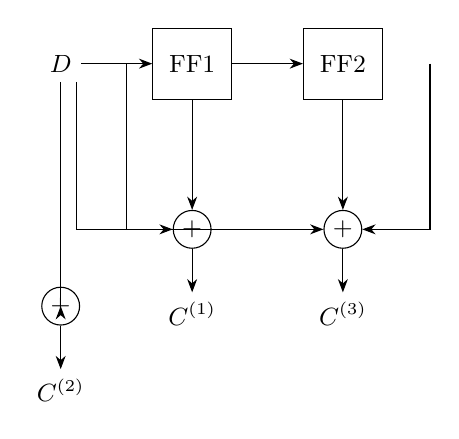
\begin{tikzpicture}[>=Stealth, font=\small,
  ff/.style={draw,minimum width=10mm,minimum height=9mm},
  xor/.style={draw,circle,inner sep=1.5pt}]
  \node (in) {$D$};
  \node[ff,right=9mm of in] (f1) {FF1};
  \node[ff,right=9mm of f1] (f2) {FF2};
  \draw[->] (in) -- (f1); \draw[->] (f1) -- (f2);
  % tap points
  \coordinate (tin) at ($(in)!0.5!(f1)$);
  \coordinate (t1)  at ($(f1.east)+(4.5mm,0)$);
  \coordinate (t2)  at ($(f2.east)+(6mm,0)$);
  % adder 1: input + FF1  (g1=110)
  \node[xor,below=14mm of f1] (a1) {$+$};
  \draw[->] (tin) |- (a1); \draw[->] (f1.south) -- (a1);
  \draw[->] (a1) -- ++(0,-8mm) node[below]{$C^{(1)}$};
  % adder 2: input only (g2=100)
  \node[xor,below=26mm of in] (a2) {$+$};
  \draw[->] ($(in.south)$) |- (a2);
  \draw[->] (a2) -- ++(0,-8mm) node[below]{$C^{(2)}$};
  % adder 3: input + FF1 + FF2 (g3=111)
  \node[xor,below=14mm of f2] (a3) {$+$};
  \draw[->] (t2) |- (a3); \draw[->] (f2.south) -- (a3);
  \draw[->] ($(in.south)+(2mm,0)$) |- (a3);
  \draw[->] (a3) -- ++(0,-8mm) node[below]{$C^{(3)}$};
\end{tikzpicture}
\end{center}

% ---------- Q7 : diagram 2 ----------
\clearpage
\section*{Q7 --- diagram 2}
\begin{center}
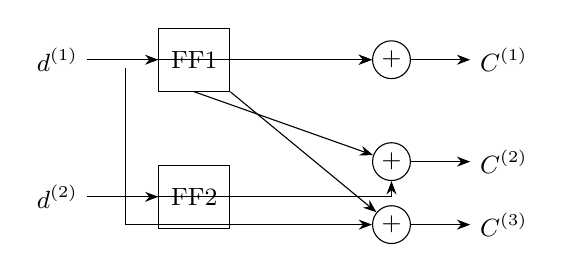
\begin{tikzpicture}[>=Stealth, font=\small,
  ff/.style={draw,minimum width=9mm,minimum height=8mm},
  xor/.style={draw,circle,inner sep=1.5pt}]
  \node (d1) {$d^{(1)}$};
  \node[ff,right=9mm of d1] (f1) {FF1};
  \node[below=12mm of d1] (d2) {$d^{(2)}$};
  \node[ff,right=9mm of d2] (f2) {FF2};
  \draw[->] (d1) -- (f1); \draw[->] (d2) -- (f2);
  \node[xor,right=18mm of f1] (a1) {$+$};   % C1 = d1 + FF1
  \draw[->] ($(d1)!0.5!(f1)$) |- (a1); \draw[->] (f1) -- (a1);
  \draw[->] (a1) -- ++(10mm,0) node[right]{$C^{(1)}$};
  \node[xor,below=8mm of a1] (a2) {$+$};     % C2 = d1 + d2 + FF1
  \draw[->] (f1.south) -- (a2);
  \draw[->] ($(d2)!0.5!(f2)$) -| (a2);
  \draw[->] (a2) -- ++(10mm,0) node[right]{$C^{(2)}$};
  \node[xor,below=16mm of a1] (a3) {$+$};    % C3 = d1 (+ FF? g=11 means d1+FF1? here 1+x)
  \draw[->] ($(d1)!0.5!(f1)+(0,-1mm)$) |- (a3); \draw[->] (f1.south east) -- (a3);
  \draw[->] (a3) -- ++(10mm,0) node[right]{$C^{(3)}$};
\end{tikzpicture}
\end{center}

% ---------- Q10 : diagram 3 ----------
\clearpage
\section*{Q10 --- diagram 3}
\begin{center}
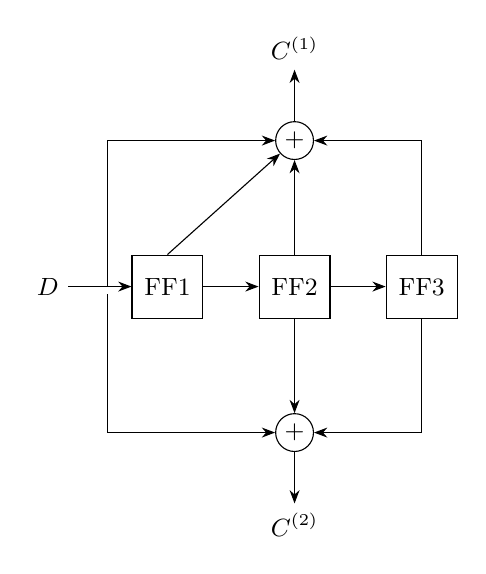
\begin{tikzpicture}[>=Stealth, font=\small,
  ff/.style={draw,minimum width=9mm,minimum height=8mm},
  xor/.style={draw,circle,inner sep=1.5pt}]
  \node (in) {$D$};
  \node[ff,right=8mm of in] (f1) {FF1};
  \node[ff,right=7mm of f1] (f2) {FF2};
  \node[ff,right=7mm of f2] (f3) {FF3};
  \draw[->] (in) -- (f1); \draw[->] (f1) -- (f2); \draw[->] (f2) -- (f3);
  % top adder C1 = in + f1 + f2 + f3
  \node[xor,above=12mm of f2] (a1) {$+$};
  \draw[->] ($(in)!0.5!(f1)$) |- (a1);
  \draw[->] (f1.north) -- (a1); \draw[->] (f2.north) -- (a1); \draw[->] (f3.north) |- (a1);
  \draw[->] (a1) -- ++(0,9mm) node[above]{$C^{(1)}$};
  % bottom adder C2 = in + f2 + f3
  \node[xor,below=12mm of f2] (a2) {$+$};
  \draw[->] ($(in)!0.5!(f1)+(0,-1mm)$) |- (a2);
  \draw[->] (f2.south) -- (a2); \draw[->] (f3.south) |- (a2);
  \draw[->] (a2) -- ++(0,-9mm) node[below]{$C^{(2)}$};
\end{tikzpicture}
\end{center}

% ---------- Q12 : diagram 4 ----------
\clearpage
\section*{Q12 --- diagram 4}
\begin{center}
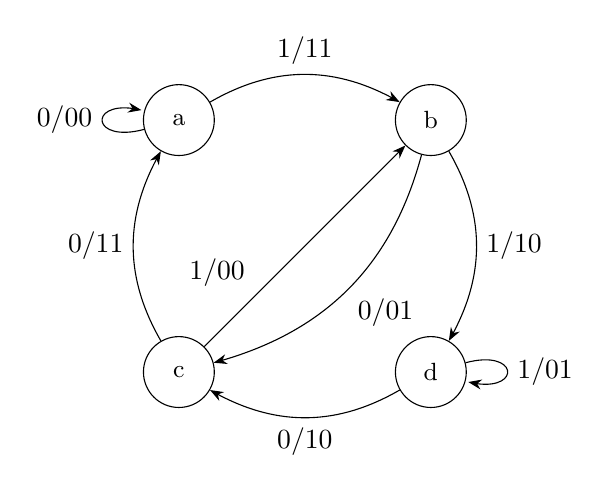
\begin{tikzpicture}[>=Stealth,node distance=3.2cm,on grid,auto,
  every state/.style={draw,minimum size=9mm,font=\small}]
  \node[state] (a) {a};
  \node[state] (b) [right=of a] {b};
  \node[state] (d) [below=of b] {d};
  \node[state] (c) [below=of a] {c};
  \path[->]
    (a) edge[loop left] node{0/00} (a)
    (a) edge[bend left] node{1/11} (b)
    (b) edge[bend left] node{0/01} (c)
    (b) edge[bend left] node{1/10} (d)
    (c) edge[bend left] node{0/11} (a)
    (c) edge node[near start]{1/00} (b)
    (d) edge[bend left] node{0/10} (c)
    (d) edge[loop right] node{1/01} (d);
\end{tikzpicture}
\end{center}

% ---------- Q12 : diagram 5 ----------
\clearpage
\section*{Q12 --- diagram 5}
\begin{center}
\begin{forest}
for tree={grow'=east, parent anchor=east, child anchor=west, edge={-Stealth},
          l sep=18mm, s sep=3mm, font=\footnotesize}
[a
  [a, edge label={node[midway,above,font=\tiny]{0/00}}
     [a, edge label={node[midway,above,font=\tiny]{0/00}}]
     [b, edge label={node[midway,below,font=\tiny]{1/11}}]]
  [b, edge label={node[midway,below,font=\tiny]{1/11}}
     [c, edge label={node[midway,above,font=\tiny]{0/01}}]
     [d, edge label={node[midway,below,font=\tiny]{1/10}}]]
]
\end{forest}
\end{center}

% ---------- Q13 : diagram 6 ----------
\clearpage
\section*{Q13 --- diagram 6}
\begin{center}
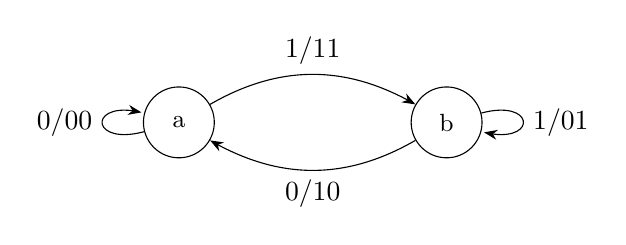
\begin{tikzpicture}[>=Stealth,node distance=3.4cm,on grid,auto,
  every state/.style={draw,minimum size=9mm,font=\small}]
  \node[state] (a) {a};
  \node[state] (b) [right=of a] {b};
  \path[->]
    (a) edge[loop left] node{0/00} (a)
    (a) edge[bend left] node{1/11} (b)
    (b) edge[bend left] node{0/10} (a)
    (b) edge[loop right] node{1/01} (b);
\end{tikzpicture}
\end{center}

% ---------- Q13 : diagram 7 ----------
\clearpage
\section*{Q13 --- diagram 7}
\begin{center}
\begin{forest}
for tree={grow'=east, parent anchor=east, child anchor=west, edge={-Stealth},
          l sep=16mm, s sep=3mm, font=\footnotesize}
[a
  [a, edge label={node[midway,above,font=\tiny]{0/00}}]
  [b, edge label={node[midway,below,font=\tiny]{1/11}}
     [a, edge label={node[midway,above,font=\tiny]{0/10}}
        [b, edge label={node[midway,below,font=\tiny]{1/11}}
           [b, edge label={node[midway,above,font=\tiny]{1/01}}
              [b, edge label={node[midway,below,font=\tiny]{1/01}}]]]]
]
\end{forest}
\end{center}

% ---------- Q14 : diagram 8 ----------
\clearpage
\section*{Q14 --- diagram 8}
\begin{center}
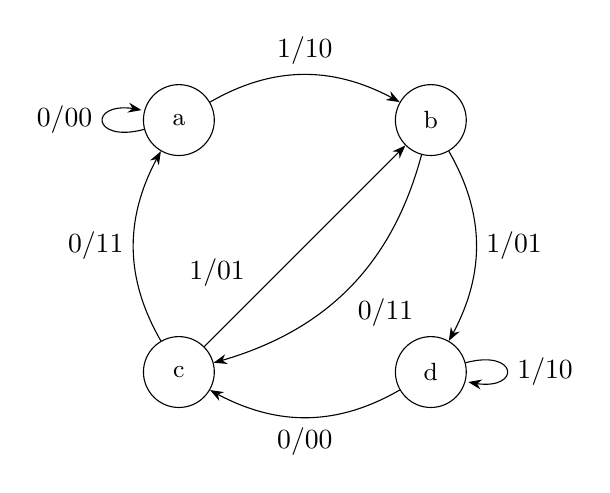
\begin{tikzpicture}[>=Stealth,node distance=3.2cm,on grid,auto,
  every state/.style={draw,minimum size=9mm,font=\small}]
  \node[state] (a) {a};
  \node[state] (b) [right=of a] {b};
  \node[state] (d) [below=of b] {d};
  \node[state] (c) [below=of a] {c};
  \path[->]
    (a) edge[loop left] node{0/00} (a)
    (a) edge[bend left] node{1/10} (b)
    (b) edge[bend left] node{0/11} (c)
    (b) edge[bend left] node{1/01} (d)
    (c) edge[bend left] node{0/11} (a)
    (c) edge node[near start]{1/01} (b)
    (d) edge[bend left] node{0/00} (c)
    (d) edge[loop right] node{1/10} (d);
\end{tikzpicture}
\end{center}

% ---------- Q15 : diagram 9 ----------
\clearpage
\section*{Q15 --- diagram 9}
\begin{center}
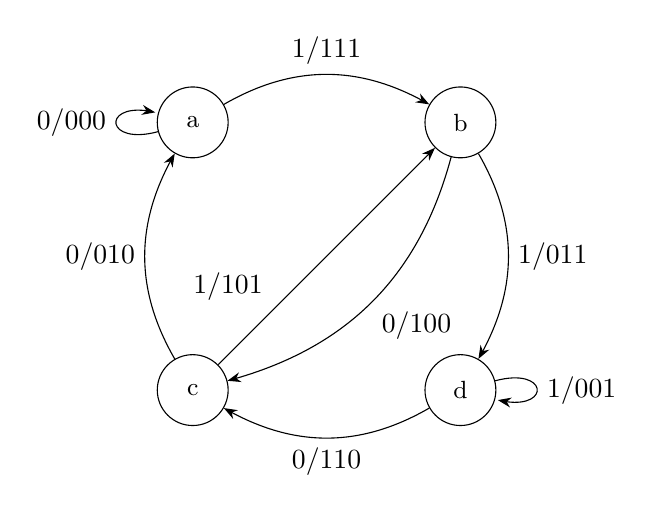
\begin{tikzpicture}[>=Stealth,node distance=3.4cm,on grid,auto,
  every state/.style={draw,minimum size=9mm,font=\small}]
  \node[state] (a) {a};
  \node[state] (b) [right=of a] {b};
  \node[state] (d) [below=of b] {d};
  \node[state] (c) [below=of a] {c};
  \path[->]
    (a) edge[loop left] node{0/000} (a)
    (a) edge[bend left] node{1/111} (b)
    (b) edge[bend left] node{0/100} (c)
    (b) edge[bend left] node{1/011} (d)
    (c) edge[bend left] node{0/010} (a)
    (c) edge node[near start]{1/101} (b)
    (d) edge[bend left] node{0/110} (c)
    (d) edge[loop right] node{1/001} (d);
\end{tikzpicture}
\end{center}

% ---------- Q15 : diagram 10 ----------
\clearpage
\section*{Q15 --- diagram 10}
\begin{center}
\begin{forest}
for tree={grow'=east, parent anchor=east, child anchor=west, edge={-Stealth},
          l sep=20mm, s sep=3mm, font=\footnotesize}
[a
  [a, edge label={node[midway,above,font=\tiny]{0/000}}
     [a, edge label={node[midway,above,font=\tiny]{0/000}}]
     [b, edge label={node[midway,below,font=\tiny]{1/111}}]]
  [b, edge label={node[midway,below,font=\tiny]{1/111}}
     [c, edge label={node[midway,above,font=\tiny]{0/100}}]
     [d, edge label={node[midway,below,font=\tiny]{1/011}}]]
]
\end{forest}
\end{center}

% ---------- Q16 : diagram 11 ----------
\clearpage
\section*{Q16 --- diagram 11}
\begin{center}
\begin{tikzpicture}[>=Stealth, font=\scriptsize, x=24mm, y=11mm]
  % states a,b,c,d at y=0,-1,-2,-3 ; stages t=0..5
  \foreach \s/\y in {a/0,b/-1,c/-2,d/-3}{
    \foreach \t in {0,...,5}{ \node[circle,fill=black,inner sep=1pt] (\s\t) at (\t,\y){};
       \ifnum\t=0 \node[left] at (\s0){\s}\fi }}
  % survivor (bold) path for message 10111: a->b->c->b->d->d
  \draw[very thick,->] (a0)--(b1) node[midway,above,sloped]{11};
  \draw[very thick,->] (b1)--(c2) node[midway,above,sloped]{10};
  \draw[very thick,->] (c2)--(b3) node[midway,above,sloped]{00};
  \draw[very thick,->] (b3)--(d4) node[midway,above,sloped]{01};
  \draw[very thick,->] (d4)--(d5) node[midway,above,sloped]{10};
  % faint full trellis branches (input 0 solid-thin, input 1 dashed)
  \foreach \t/\tn in {0/1,1/2,2/3,3/4,4/5}{
    \draw[gray!40] (a\t)--(a\tn); \draw[gray!40,dashed] (a\t)--(b\tn);
    \draw[gray!40] (b\t)--(c\tn); \draw[gray!40,dashed] (b\t)--(d\tn);
    \draw[gray!40] (c\t)--(a\tn); \draw[gray!40,dashed] (c\t)--(b\tn);
    \draw[gray!40] (d\t)--(c\tn); \draw[gray!40,dashed] (d\t)--(d\tn);}
\end{tikzpicture}
\end{center}

% ---------- Q19 : diagram 12 ----------
\clearpage
\section*{Q19 --- diagram 12}
\begin{center}
\begin{tikzpicture}[>=Stealth, font=\scriptsize, x=26mm, y=11mm]
  \foreach \s/\y in {a/0,b/-1,c/-2,d/-3}{
    \foreach \t in {0,...,5}{ \node[circle,fill=black,inner sep=1pt] (\s\t) at (\t,\y){};
       \ifnum\t=0 \node[left] at (\s0){\s}\fi }}
  % received groups along the top
  \foreach \t/\r in {1/11,2/00,3/00,4/01,5/11}{ \node[above] at (\t-0.5,0.6){\r}; }
  % faint full trellis
  \foreach \t/\tn in {0/1,1/2,2/3,3/4,4/5}{
    \draw[gray!35] (a\t)--(a\tn); \draw[gray!35,dashed] (a\t)--(b\tn);
    \draw[gray!35] (b\t)--(c\tn); \draw[gray!35,dashed] (b\t)--(d\tn);
    \draw[gray!35] (c\t)--(a\tn); \draw[gray!35,dashed] (c\t)--(b\tn);
    \draw[gray!35] (d\t)--(c\tn); \draw[gray!35,dashed] (d\t)--(d\tn);}
  % survivor path a->b->c->a->b->a  (message 1 0 1 0 0)
  \draw[very thick,->] (a0)--(b1);
  \draw[very thick,->] (b1)--(c2);
  \draw[very thick,->] (c2)--(a3);
  \draw[very thick,->] (a3)--(b4);
  \draw[very thick,->] (b4)--(a5);
  \node[below=6mm] at (2.5,-3){decoded message $=10100$, final metric $=1$};
\end{tikzpicture}
\end{center}
\end{document}
